\chapter{Specifikacija programske potpore}
		
	\section{Funkcionalni zahtjevi}
			
			\noindent \textbf{Dionici:}
			
			\begin{packed_enum}
				
				\item Administrator
				\item Seizmolozi
				\item Građani (neregistrirani korisnici)
				\item Razvojni tim

			\end{packed_enum}
			
			\noindent \textbf{Aktori i njihovi funkcionalni zahtjevi:}
			
			
			\begin{packed_enum}
				\item  \underbar{Neregistrirani/neprijavljeni korisnik (građanin) može:}
				
				\begin{packed_enum}
					
					\item ispuniti upitnik ako je osjetio novi potres
					\item pregledati sve arhivirane potrese s:
					\begin{packed_enum}

						\item interaktivnom kartom Hrvatske 
						\item dodatnim informacijama (broj ispunjenih upitnika, datum, vrijeme, geografski položaj, dubina fokusa, magnituda i naziv područja)
					
					\end{packed_enum}
					\item pristupiti aktualnim potresima i:
					\begin{packed_enum}

						\item ispuniti upitnik
						\item pregledati već analizirane podatke (karta, datum, vrijeme, itd.)
					
					\end{packed_enum}
				\end{packed_enum}
			
				\item  \underbar{Administrator može:}
				
				\begin{packed_enum}

					\item sve što i neregistrirani/neprijavljeni korisnik može
					\item stvoriti novi potres od jednog ili više upitnika
					\item dodati upitnik nekom od postojećih potresa
					\item registrirati nove seizmologe
					\item ukloniti registrirane seizmologe
					\item preuzeti podatke o potresu
					\item izmijeniti svoje podatke
					
				\end{packed_enum}

				\item  \underbar{Seizmolog/znanstvenik može:}

				\begin{packed_enum}

					\item pristupiti aplikaciji nakon prijave (e-mail i lozinka)
					\item pregledavati podatke o:
					\begin{packed_enum}
						
						\item arhiviranim potresima
						\item aktualnim potresima

					\end{packed_enum}
					\item u tekstualnom formatu preuzeti podatke o potresima
					\item izmijeniti svoje podatke
				\end{packed_enum}
			\end{packed_enum}
			
			\eject 
			
			
				
			\subsection{Obrasci uporabe}
				
				\subsubsection{Opis obrazaca uporabe}					

					\noindent \underbar{\textbf{UC1 - Prijava}}
					\begin{packed_item}
	
						\item \textbf{Glavni sudionik:} Korisnik (seizmolog, administrator)
						\item \textbf{Cilj:} Dobiti pristup odgovarajućem sučelju na temelju uloge i ovlastima
						\item \textbf{Sudionici:} Baza podataka
						\item \textbf{Preduvjet:} Registracija
						\item \textbf{Opis osnovnog tijeka:}
						
						\item[] \begin{packed_enum}
	
							\item Korisnik odabire opciju za prijavu
							\item Pokazuje se obrazac za prijavu
							\item Korisnik unosi korisničke podatke (e-mail, lozinka)
							\item Provjera ispravnosti unesenih podataka
							\item Pristup odgovarajućim funkcijama
						\end{packed_enum}
						
						\item  \textbf{Opis mogućih odstupanja:}
						
						\item[] \begin{packed_item}
	
							\item[4.a] Neispravan email ili lozinka
							\item[] \begin{packed_enum}
								
								\item Sustav obavještava korisnika o netočnim informacijama
								\item Sustav vraća korisnika na obrazac za prijavu
								
							\end{packed_enum}
							
						\end{packed_item}
					\end{packed_item}

					\noindent \underbar{\textbf{UC2 - Registracija novih seizmologa}}
					\begin{packed_item}
	
						\item \textbf{Glavni sudionik:} Administrator
						\item \textbf{Cilj:} Registrirati nove seizmologe
						\item \textbf{Sudionici:} Seizmolog, Baza podataka
						\item \textbf{Preduvjet:} Administrator prijavljen
						\item \textbf{Opis osnovnog tijeka:}
						
						\item[] \begin{packed_enum}
	
							\item Administrator na svom profilu odabire opciju "Registriraj seizmologa"
							\item Pokazuje se obrazac za registraciju
							\item Administrator unosi korisničke podatke (ime, prezime, e-mail, lozinka)
							\item Administrator potvrđuje unos
							\item Baza podataka se ažurira
							\item Seizmolog dobiva e-mail obavijest o registraciji
						
						\end{packed_enum}
						
						\item  \textbf{Opis mogućih odstupanja:}
						
						\item[] \begin{packed_item}
	
							\item[3.a] Unos neispravnog e-maila
							\item[] \begin{packed_enum}
								
								\item Sustav obavještava administratora o neispravnom upisu e-maila i vraća ga na stranicu za registraciju
								\item Administrator mijenja potrebne podatke te završava unos ili odustaje od registracije
								
							\end{packed_enum}							
						\end{packed_item}
					\end{packed_item}

					\noindent \underbar{\textbf{UC3 - Pregled korisničkih podataka}}
					\begin{packed_item}
	
						\item \textbf{Glavni sudionik:} Seizmolog, Administrator
						\item \textbf{Cilj:} Pregled podataka
						\item \textbf{Sudionici:} Baza podataka
						\item \textbf{Preduvjet:} Korisnik prijavljen u sustav
						\item  \textbf{Opis osnovnog tijeka:}
						
						\item[] \begin{packed_enum}
	
							\item Korisnik u kutu početne stranice odabire opciju za pregled profila
							\item Korisnik pregledava podatke

						\end{packed_enum}						
					\end{packed_item}

					\noindent \underbar{\textbf{UC4 - Promjena korisničkih podataka}}
					\begin{packed_item}
	
						\item \textbf{Glavni sudionik:} Administrator, Seizmolog
						\item \textbf{Cilj:} Promjena podataka
						\item \textbf{Sudionici:} Baza podataka
						\item \textbf{Preduvjet:} Korisnik prijavljen u sustav 
						\item  \textbf{Opis osnovnog tijeka:}
						
						\item[] \begin{packed_enum}
	
							\item Pregled profila
							\item Odabir opcije za promjenu podataka
							\item Korisnik mijenja željene podatke
							\item Korisnik potvrđuje promjenu
							\item Ažurira se baza podataka
							
						\end{packed_enum}
					\end{packed_item}

					\noindent \underbar{\textbf{UC5 - Uklanjanje seizmologa}}
					\begin{packed_item}
	
						\item \textbf{Glavni sudionik:} Administrator
						\item \textbf{Cilj:} Uklanjanje registriranih seizmologa iz sustava
						\item \textbf{Sudionici:} Baza podataka, Seizmolog
						\item \textbf{Preduvjet:} 
							\begin{packed_item}
								\item Administrator prijavljen u sustav
								\item Postojanje barem jednog registriranog seizmologa
							\end{packed_item}
						\item  \textbf{Opis osnovnog tijeka:}
						
						\item[] \begin{packed_enum}
	
							\item Pregled seizmologa
							\item Odabir opcije "Ukloni" pored imena seizmologa
							\item Sustav obavještava administratora o uklanjanju seizmologa
							\item Sustav šalje e-mail obavijest seizmologu da je uklonjen iz sustava
							\item Ažuriranje baze podataka
							
						\end{packed_enum}
					\end{packed_item}

					\noindent \underbar{\textbf{UC6 - Pregled seizmologa}}
					\begin{packed_item}
	
						\item \textbf{Glavni sudionik:} Administrator
						\item \textbf{Cilj:} Pregled seizmologa koji su registrirani u sustavu
						\item \textbf{Sudionici:} Baza podataka
						\item \textbf{Preduvjet:} Administrator prijavljen u sustav
						\item \textbf{Opis osnovnog tijeka:}
						
						\item[] \begin{packed_enum}
	
							\item Administrator u izborniku na početnoj stranici odabire opciju za pregled profila
							\item Administrator na profilu odabire opciju "Pregledaj seizmologe"
							\item Sustav prikazuje popis registriranih korisnika (seizmologa)
							
						\end{packed_enum}
						
						\item  \textbf{Opis mogućih odstupanja:}
						
						\item[] \begin{packed_item}
	
							\item[2.a] Nema registriranih seizmologa
							\item[] \begin{packed_enum}
								
								\item Prikazuje se poruka da još nema registriranih seizmologa
								
							\end{packed_enum}
							
						\end{packed_item}
					\end{packed_item}

					\noindent \underbar{\textbf{UC7 - Pregled upitnika}}
					\begin{packed_item}
	
						\item \textbf{Glavni sudionik:} Administrator
						\item \textbf{Cilj:} Pregled pristiglih upitnika
						\item \textbf{Sudionici:} Baza podataka
						\item \textbf{Preduvjet:} Administrator prijavljen u sustav
						\item \textbf{Opis osnovnog tijeka:}
						
						\item[] \begin{packed_enum}
	
							\item Administrator u izborniku na početnoj stranici odabire opciju za pregled profila
							\item Administrator na profilu odabire opciju "Pregledaj nove upitnike"
							\item Sustav prikazuje popis pristiglih upitnika
							
						\end{packed_enum}
						
						\item  \textbf{Opis mogućih odstupanja:}
						
						\item[] \begin{packed_item}
	
							\item[2.a] Nema novih upitnika
							\item[] \begin{packed_enum}
								
								\item Prikazuje se poruka da nema upitnika
								
							\end{packed_enum}
							
						\end{packed_item}
					\end{packed_item}

					\noindent \underbar{\textbf{UC8 - Registracija novog potresa}}
					\begin{packed_item}
	
						\item \textbf{Glavni sudionik:} Administrator
						\item \textbf{Cilj:} Stvoriti novi aktualni potres
						\item \textbf{Sudionici:} Baza podataka
						\item \textbf{Preduvjet:} 
						\begin{packed_item}
							\item Administrator prijavljen u sustav
							\item Postojanje upitnika
						\end{packed_item}
						            
						\item \textbf{Opis osnovnog tijeka:}
						
						\item[] \begin{packed_enum}
	
							\item Pregled pristiglih upitnika
							\item Odabir jednog ili više upitnika
							\item Odabir „Dodaj novi potres“ u izborniku
							\item Otvara se obrazac za dodavanje novog potresa
							\item Administrator unosi naziv potresa
							\item Administrator odabire opciju "Potvrdi" čime potvrđuje unos novog potresa
							\item Ažurira se baza podataka
							\item Sustav obavještava administratora o uspješnosti dodavanja novog potresa
							
						\end{packed_enum}
					\end{packed_item}

					\noindent \underbar{\textbf{UC9 - Dodavanje upitnika postojećem aktualnom potresu}}
					\begin{packed_item}
	
						\item \textbf{Glavni sudionik:} Administrator
						\item \textbf{Cilj:} Svrstavanje upitnika već postojećim potresima u svrhu upotpunjavanja informacija
						\item \textbf{Sudionici:} Baza podataka
						\item \textbf{Preduvjet:} 
						\begin{packed_item}
							\item Administrator prijavljen u sustav
							\item Postojanje upitnika
							\item Postojanje aktualnog potresa
						\end{packed_item}

						\item \textbf{Opis osnovnog tijeka:}
						
						\item[] \begin{packed_enum}
	
							\item Pregled pristiglih upitnika
							\item Odabir jednog ili više upitnika
							\item Odabir nekog imenovanog potresa iz izbornika
							\item Baza podataka se ažurira
							\item Sustav obavještava administratora o uspješnosti dodavanja upitnika postojećem potresu
							
						\end{packed_enum}
					\end{packed_item}

					\noindent \underbar{\textbf{UC10 - Brisanje upitnika}}
					\begin{packed_item}
	
						\item \textbf{Glavni sudionik:} Administrator
						\item \textbf{Cilj:} Ukloniti nerelevantne upitnike
						\item \textbf{Sudionici:} Baza podataka
						\item \textbf{Preduvjet:} 
						\begin{packed_item}
							\item Administrator prijavljen u sustav
							\item Postojanje upitnika
						\end{packed_item}

						\item \textbf{Opis osnovnog tijeka:}
						
						\item[] \begin{packed_enum}
	
							\item Pregled pristiglih upitnika
							\item Odabir jednog ili više upitnika
							\item Odabir „Obriši“
							\item Brišu se upitnici iz baze podataka
							\item Sustav obavještava administratora o uspješnosti brisanja upitnika
							
						\end{packed_enum}
					\end{packed_item}

					\noindent \underbar{\textbf{UC11 - Arhiviranje aktualnih potresa}}
					\begin{packed_item}
	
						\item \textbf{Glavni sudionik:} Administrator
						\item \textbf{Cilj:} Prebaciti aktualne potrese u kategoriju arhiviranih
						\item \textbf{Sudionici:} Baza podataka
						\item \textbf{Preduvjet:} 
						\begin{packed_item}
							\item Administrator prijavljen u sustav
							\item Postojanje aktualnih potresa
						\end{packed_item}

						\item \textbf{Opis osnovnog tijeka:}
						
						\item[] \begin{packed_enum}
	
							\item Pregled aktualnih potresa
							\item Odabir jednog ili više aktualnih potresa
							\item Odabir „Arhiviraj“
							\item Baza podataka se ažurira
							\item Sustav obavještava korisnika o uspješnosti arhiviranja potresa
							
						\end{packed_enum}
					\end{packed_item}

					\noindent \underbar{\textbf{UC12 - Pregled aktualnih potresa}}
					\begin{packed_item}
	
						\item \textbf{Glavni sudionik:} Administrator
						\item \textbf{Cilj:} Prebaciti aktualne potrese u kategoriju arhiviranih
						\item \textbf{Sudionici:} Baza podataka
						\item \textbf{Preduvjet:} -

						\item \textbf{Opis osnovnog tijeka:}
						
						\item[] \begin{packed_enum}
							\item Na početnoj stranici odabir opcije „Aktualni potresi“
							\item Prilikom učitavanja stranice prikazana je preliminarna karta intenziteta i popis aktualnih potresa
						\end{packed_enum}
						
						\item  \textbf{Opis mogućih odstupanja:}
						
						\item[] \begin{packed_item}
	
							\item[2.a] Nema aktualnih potresa
							\item[] \begin{packed_enum}
								
								\item Prikazuje se odgovarajuća poruka
								
							\end{packed_enum}
							
						\end{packed_item}
						
					\end{packed_item}

					\noindent \underbar{\textbf{UC13 - Odjava iz sustava}}
					\begin{packed_item}
	
						\item \textbf{Glavni sudionik:} Seizmolog, Administrator
						\item \textbf{Cilj:} Odjaviti se iz sustava
						\item \textbf{Sudionici:} Baza podataka
						\item \textbf{Preduvjet:} Korisnik prijavljen u sustav

						\item \textbf{Opis osnovnog tijeka:}
						
						\item[] \begin{packed_enum}
							\item Odabir opcije za odjavu
							\item Korisnik se odjavljuje iz sustava
							\item Prikazuje se početna stranica za neregistriranog korisnika
						\end{packed_enum}
					\end{packed_item}

			\noindent \underbar{\textbf{UC14 - Preuzimanje podataka o arhiviranim potresima}}
			\begin{packed_item}
				
				\item \textbf{Glavni sudionik:} Seizmolog, Administrator
				\item \textbf{Cilj:} Preuzimanje podataka o potresima
				\item \textbf{Sudionici:} Baza podataka
				\item \textbf{Preduvjet:} Korisnik prijavljen u sustav
				
				\item \textbf{Opis osnovnog tijeka:}
				
				\item[] \begin{packed_enum}
					\item Pregled i pretraživanje/filtriranje arhiviranih potresa
					\item Odabir željenih potresa
					\item Odabir opcije „Preuzmi“
					\item Preuzimanje podatak
				\end{packed_enum}
			\end{packed_item}
			
			\noindent \underbar{\textbf{UC15 - Preuzimanje podataka o aktualnim potresima}}
			\begin{packed_item}
				
				\item \textbf{Glavni sudionik:} Seizmolog, Administator
				\item \textbf{Cilj:} Preuzimanje podataka o potresima
				\item \textbf{Sudionici:} Baza podataka
				\item \textbf{Preduvjet:} Korisnik prijavljen u sustav
				
				\item \textbf{Opis osnovnog tijeka:}
				
				\item[] \begin{packed_enum}
					\item Pregled i pretraživanje/filtriranje arhiviranih potresa
					\item Odabir željenih potresa
					\item Odabir opcije „Preuzmi“
					\item Preuzimanje podataka
				\end{packed_enum}
				
				\item  \textbf{Opis mogućih odstupanja:} -
				
			\end{packed_item}
			
			\noindent \underbar{\textbf{UC16 - Pregled arhiviranih potresa}}
			\begin{packed_item}
				
				\item \textbf{Glavni sudionik:} Korisnik (neregistrirani građanih, seizmolog, administrator)
				\item \textbf{Cilj:} Pregledati arhivirane potrese
				\item \textbf{Sudionici:} Baza podataka
				\item \textbf{Preduvjet:} -
				
				\item \textbf{Opis osnovnog tijeka:}
				
				\item[] \begin{packed_enum}
					\item Na početnoj stranici odabir opcije „Arhivirani potresi“
					\item Prilikom učitavanja stranice prikazana je preliminarna karta intenziteta i popis arhiviranih potresa
				\end{packed_enum}
				
				\item  \textbf{Opis mogućih odstupanja:}
				
				\item[] \begin{packed_item}
					
					\item[2.a] Nema arhiviranih potresa
					\item[] \begin{packed_enum}
						
						\item Prikazuje se odgovarajuća poruka da još nema arhiviranih potresa
						
					\end{packed_enum}
					
				\end{packed_item}
				
			\end{packed_item}
			
			\noindent \underbar{\textbf{UC17 - Pretraživanje/filtriranje arhiviranih potresa}}
			\begin{packed_item}
				
				\item \textbf{Glavni sudionik:} Korisnik (neregistrirani građanin, seizmolog, administrator)
				\item \textbf{Cilj:} Pretražiti i filtrirati arhivirane potrese
				\item \textbf{Sudionici:} Baza podataka
				\item \textbf{Preduvjet:} -
				
				\item \textbf{Opis osnovnog tijeka:}
				
				\item[] \begin{packed_enum}
					\item Na početnoj stranici odabir opcije „Arhivirani potresi“
					\item Prilikom učitavanja stranice prikazana je preliminarna karta intenziteta i popis arhiviranih potresa
					\item Korisnik pretražuje ili filtrira po mjestu, vremenu i intenzitetu
					\item Pregled potresa s traženim svojstvima
				\end{packed_enum}
				
				\item  \textbf{Opis mogućih odstupanja:}
				
				\item[] \begin{packed_item}
					
					\item[3.a] Korisnik pri pretraživanju upisuje podatke koji nisu važeći ni za jedan arhivirani potres
					\item[] \begin{packed_enum}
						
						\item Ne prikazuje ni jedan arhivirani potres na karti ni na popisu
						\item Ispisuje se poruka da nije pronađen ni jedan potres
						
					\end{packed_enum}
					
				\end{packed_item}
				
			\end{packed_item}
			\noindent \underbar{\textbf{UC18 - Pretraživanje/filtriranje aktualnih potresa}}
			\begin{packed_item}
				
				\item \textbf{Glavni sudionik:} Korisnik (neregistrirani građanin, seizmolog, administrator)
				\item \textbf{Cilj:} Pretražiti i filtrirati aktualne potrese
				\item \textbf{Sudionici:} Baza podataka
				\item \textbf{Preduvjet:} -
				
				\item \textbf{Opis osnovnog tijeka:}
				
				\item[] \begin{packed_enum}
					\item Na početnoj stranici odabir opcije „Aktualni potresi“
					\item Prilikom učitavanja stranice prikazana je preliminarna karta intenziteta i popis aktualnih potresa
					\item Korisnik pretražuje ili filtrira po mjestu, vremenu i intenzitetu
					\item Pregled potresa s traženim svojstvima
				\end{packed_enum}
				
				\item  \textbf{Opis mogućih odstupanja:}
				
				\item[] \begin{packed_item}
					
					\item[3.a] Korisnik pri pretraživanju upisuje podatke koji nisu važeći ni za jedan aktualni potres
					\item[] \begin{packed_enum}
						
						\item Ne prikazuje ni jedan aktualni potres na karti ni na popisu
						\item Ispisuje se poruka da nije pronađen ni jedan potres
						
					\end{packed_enum}
					
				\end{packed_item}
				
			\end{packed_item}	
			
			\noindent \underbar{\textbf{UC19 - Prijava novog potresa}}
			\begin{packed_item}
				
				\item \textbf{Glavni sudionik:} Korisnik (neregistrirani građanin, seizmolog, administrator)
				\item \textbf{Cilj:} Ispuniti upitnik kako bi se prijavio novi potres
				\item \textbf{Sudionici:} Baza podataka
				\item \textbf{Preduvjet:} -
				
				\item \textbf{Opis osnovnog tijeka:}
				
				\item[] \begin{packed_enum}
					\item Na početnoj stranici odabir opcije „Novi potres?“
					\item Otvorena se upitnik
					\item Korisnik ispunjava upitnik
					\item Odabir opcije "Predaj"
					\item Dodaje se novi potres u bazu podataka
					\item Korisnik dobiva povratnu informaciju da je uspješno ispunio upitnik
				\end{packed_enum}
				
				\item  \textbf{Opis mogućih odstupanja:}
				
				\item[] \begin{packed_item}
					
					\item[3.a] Korisnik nije odgovorio na obvezno pitanje
					\item[] \begin{packed_enum}
						
						\item Sustav obavještava korisnika o neuspjeloj predaji te ga vraća na stranicu s upitnikom						
					\end{packed_enum}
					
					\item[4.a] Odabir opcije "Odustani"
					\item[] \begin{packed_enum}
						
						\item Podaci nisu sačuvani
						\item Sustav vraća korisnika na početnu stranicu						
					\end{packed_enum}
					
				\end{packed_item}
				
			\end{packed_item}
			
			\noindent \underbar{\textbf{UC20 - Ispunjavanje upitnika za aktualni potres}}
			\begin{packed_item}
				
				\item \textbf{Glavni sudionik:} Korisnik (neregistrirani građanin, seizmolog, administrator)
				\item \textbf{Cilj:} Ispuniti upitnik za aktualni potres
				\item \textbf{Sudionici:} Baza podataka
				\item \textbf{Preduvjet:} Postojanje aktualnog potresa
				
				\item \textbf{Opis osnovnog tijeka:}
				
				\item[] \begin{packed_enum}
					\item Na početnoj stranici odabir opcije „Aktualni potresi“
					\item Pregled aktualnih potresa
					\item Odabir željenog aktualnog potresa
					\item Odabir opcije "Ispuni upitnik"
					\item Otvara se upitnik s popunjenim mjestom, datumom i vremenom odabranog aktualnog potresa
					\item Korisnik ispunjava ostatak upitnika
					\item Odabir opcije "Predaj"
					\item Dodavanje informacija iz upitnika u bazu podataka
					\item Ažuriranje podataka o aktualnom potresu
					\item Korisnik dobiva povratnu informaciju da je uspješno ispunio upitnik
				\end{packed_enum}
				
				\item  \textbf{Opis mogućih odstupanja:}
				
				\item[] \begin{packed_item}
					
					\item[6.a] Korisnik nije odgovorio na obvezno pitanje
					\item[] \begin{packed_enum}
						
						\item Sustav obavještava korisnika o neuspjeloj predaji te ga vraća na stranicu s upitnikom
						
					\end{packed_enum}
					
					\item[7.a] Odabir opcije "Odustani"
					\item[] \begin{packed_enum}
						
						\item Podaci nisu sačuvani
						\item Sustav vraća korisnika na stranicu aktualnih potresa
						
					\end{packed_enum}
					
				\end{packed_item}
				
			\end{packed_item}						
					
				\subsubsection{Dijagrami obrazaca uporabe}
					
				\begin{figure}[H]
					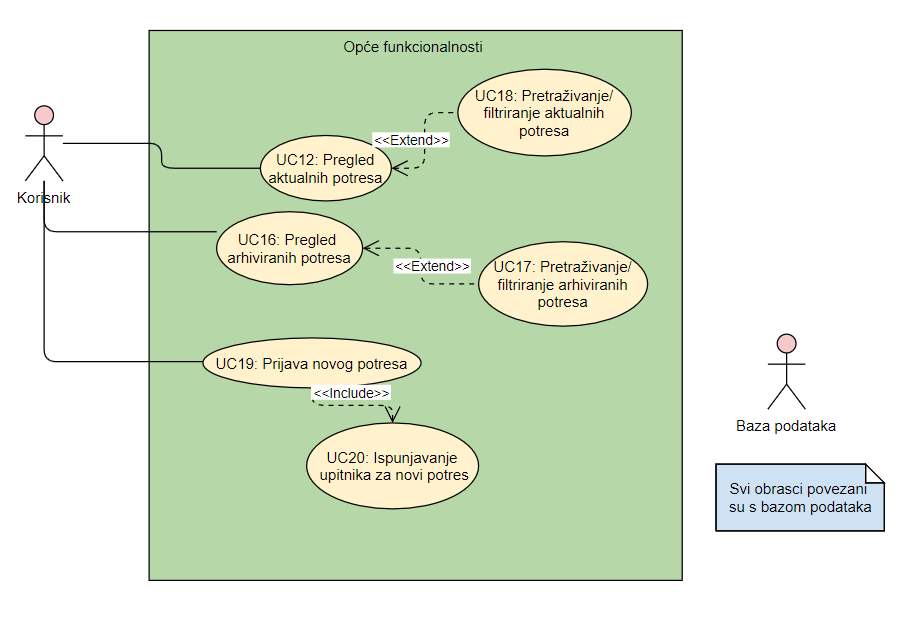
\includegraphics[width=\textwidth, height = 15cm]{slike/prvinovo.PNG} 
					 \caption{Dijagram obrazaca uporabe, funkcionalnosti koje imaju svi korisnici}
					  \label{fig:obrasci1} 
				  \end{figure}
				  
				  \begin{figure}[H]
					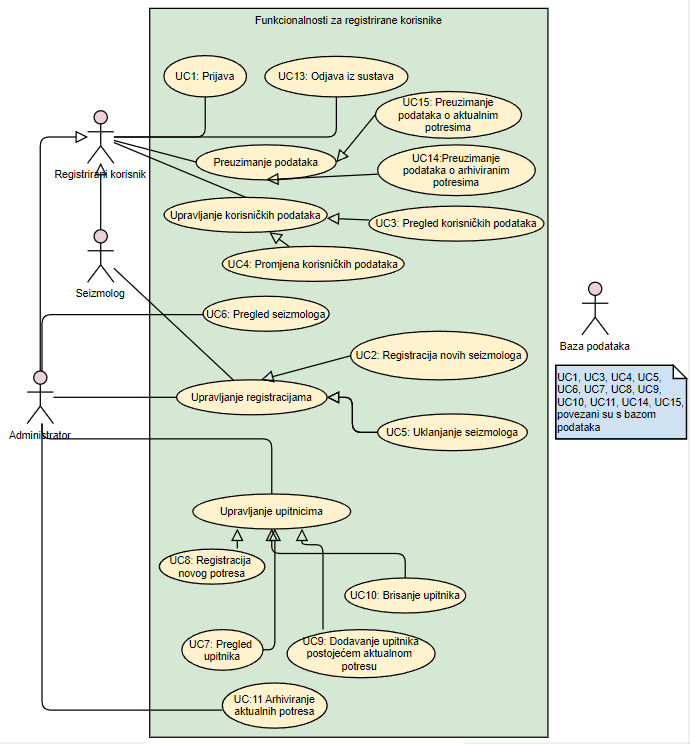
\includegraphics[width=\textwidth]{slike/druginovo.PNG} 
					\caption{Dijagram obrazaca uporabe, funkcionalnosti koje imaju regestrirani korisnici}
					\label{fig:obrasci2} 
				   \end{figure}
				\eject		
				
			\subsection{Sekvencijski dijagrami}
				
			\textbf{UC4: Potvrđivanje novih registracija}\\
			{Administrator odabire opciju "Zahtjevi za registraciju". Poslužitelj potom šalje zahtjev za dohvaćanjem svih zahtjeva za registraciju bazi podataka. Zahtjev se prihvaća te se vraća popis onih korisnika koji se žele registrirati za seizmologa. Popis se prikazuje na klijentu. Administrator može označiti željene korisnike te potom pritisnuti "Potvrdi". Time su zahtjevi obrađeni te se u bazi označenim korisnicima uloga mijenja u "seizmolog". Sustav obavijesti administratora o uspješnom dodavanju seizmologa. Novim seizmolozima se šalje e-mail kako bi ih se obavijestilo da je njihova registracija potvrđena.}
			\begin{figure}[H]
				  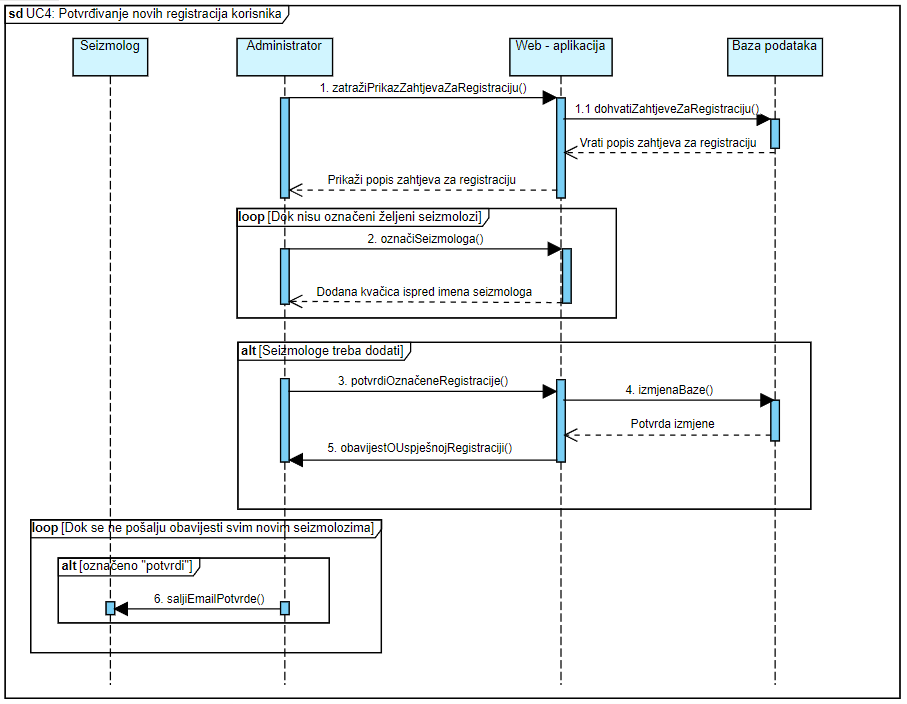
\includegraphics[width=\textwidth, height=14cm]{slike/uc4.PNG}
				  \caption{sekvencijski dijagram za UC4}
				  \label{fig:sekvuc4} 
				 \end{figure}
			\textbf{UC20: Ispunjavanje upitnika za aktualni potres}\\
			{Korisnik odabire opciju "Aktualni potresi". Poslužitelj potom šalje zahtjev bazi podataka kako bi dohvatio sve aktualne potrese. Prihvaća se zahtjev te se na klijentu prikazuju svi aktualni potresi. Korisnik odabire potres za koji želi ispuniti upitnik. S klijenta se bazi podataka šalje zahtjev za dohvaćanjem podataka o potresu koji se automatski popunjavaju u upitniku. Korisniku se prikazuje upitnik s djelomično popunjenim odgovorima. Korisnik popunjava upitnik. Kada pritisne opciju "Predaj", upitnik se šalje na validaciju. Ako su odgovorena sva pitanja, odgovori se pohranjuju u bazu te se na temelju odgovora računa intezitet potresa pa se i to ažurira u bazi. 
			Kada je upitnik uspješno predan, sustav o tome obavijesti korisnika. Ako nije sve odgovoreno, korisnik dobiva obavijest o neuspjeloj predaji te ga sustav vraća na stranicu s upitnikom. Ako je korisnik odabrao "Odustani" umjesto "Predaj" sustav ga vraća na stranicu "Aktualni potresi".}
			\begin{figure}[H]
				  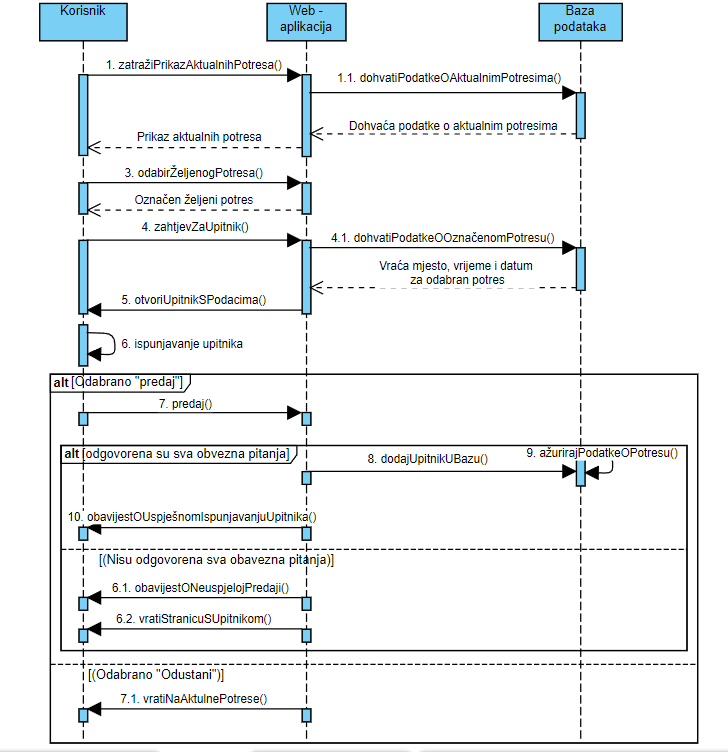
\includegraphics[width=\textwidth, height=13cm]{slike/uc20.PNG}
				  \caption{sekvencijski dijagram za UC20}
				  \label{fig:sekvuc8} 
				 \end{figure}
				\eject
	
		\section{Ostali zahtjevi}
				\begin{packed_item}
					\item Aplikacija treba podržavati rad više korisnika u stvarnom vremenu.
					\item Sustav treba biti implementiran kao mobilna ili web aplikacija koristeći objektno orijentirane jezike.
					\item Neposredno nakon što se dogodi neki potres, administrator može poslati notifikaciju na uređaje građana da ispune upitnik.
					\item Treba kreirati administratora i dva znanstvenika te barem jedan stari potres s 10 popunjenih upitnika i jedan novi potres s 5 popunjenih upitnika.
					\item Korisničko sučelje mora biti pisano na hrvatskom jeziku i podržavati dijakritičke znakove.
					\item Upitnik o potresu mora imati barem 10 pitanja pomoću kojih se može odrediti intenzitet potresa.
					\item Aplikacija mora jednostavno prikazivati informacije o potresima korisnicima.
					\item Karta treba prikazivati sve gradove i mjesta u kojima su upitnici popunjeni.
					\item Karta treba prikazivati podatke samo s jednog potresa, ne svih koji su se do sad dogodili.
				\end{packed_item}